\scanpage{36}
\mspage{3}
a) \(K^\sigma=K\) --- one thus finds the real points of \(M_{0,5}^{!}\simeq\mathrm{Sym}_2^*(\unsure{U_{0,3}|M_{0,3}})\),
\deleted{\unsure{The case|a case}} of real dimension \(2\) : contains the case \(1^\circ\) (pentagonal)

b) \(\operatorname{card}K^\sigma=3\). Taking \(0,1,\infty\) in \(K^\sigma\) as reference frame, one finds that
\[
K=\{0,1,\infty,\lambda,\bar\lambda\},\quad
\lambda\in\text{Poincaré half-plane},\quad\text{real dimension }2.
\]
Contains the case \(3^\circ\) (bitetrahedral)
\margin{One may assume \(\sigma z=\bar z\) \deleted{\unsure{for \(\nu=3\)}}}

c) \(\operatorname{card}K^\sigma=1\), that is \deleted{\unsure{?}} \(K^\sigma=\{P\}\), \inserted{Let \(K\setminus K^\sigma=I\)}, \deleted{one takes \unsure{as reference frame} \(\infty\), and one chooses a point \(0\) such that \(0=\sigma0\). One may}
\((\Sigma,I)\) is a system of \(4\) points on a complex sphere, \deleted{equipped with an} \inserted{\unsure{admitting}} an involutive antiautomorphism \deleted{\(\unsure{\sigma}\)} (``conjugation''), they are well known and of \uline{real} modular dimension \(1\), moreover the choice of an additional real point \(P\) makes one more dimension, that is total real dimension \(2\) again.
(contains the square pyramidal case, \(2^\circ\))

\figure{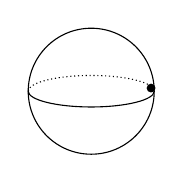
\begin{tikzpicture}[scale=.8]
\draw(0,0)circle(1);
\draw(-1,0)arc[start angle=180,end angle=360,x radius=1,y radius=.25];
\draw[densely dotted](-1,0)arc[start angle=180,end angle=0,x radius=1,y radius=.25];
\fill(.95,.05)circle(2pt);
\end{tikzpicture}}

\sbox{180}{\figure{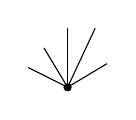
\begin{tikzpicture}[scale=.5]\fill(0,0)circle(3pt);\foreach \x/\y in {-1/.5,-.6/1,0/1.5,.7/1.5,1/.6}{\draw(0,0)--(\x,\y);}\end{tikzpicture}}}
\sbox{181}{\figure{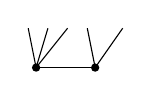
\begin{tikzpicture}[scale=.5]\draw(0,0)--(1.5,0);\fill(0,0)circle(3pt);\fill(1.5,0)circle(3pt);\draw(0,0)--(-.2,1);\draw(0,0)--(.3,1);\draw(0,0)--(.8,1);\draw(1.5,0)--(1.3,1);\draw(1.5,0)--(2.2,1);\end{tikzpicture}}}
\sbox{182}{\figure{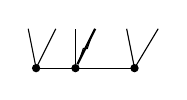
\begin{tikzpicture}[scale=.5]\draw(0,0)--(1,0)--(2.5,0);\foreach \x in {0,1,2.5}{\fill(\x,0)circle(3pt);}\draw(0,0)--(-.2,1);\draw(0,0)--(.5,1);\draw(1,0)--(1,1);\draw[thick](1.05,.1)--(1.5,1);\draw(1.1,.2)--(1.2,.5)--(1.3,.5)--(1.4,.8);\draw(2.5,0)--(2.3,1);\draw(2.5,0)--(3.1,1);\end{tikzpicture}}}
\diagram{\begin{tikzcd}[ampersand replacement=\&,column sep=large,row sep=large]
\text{modular dimension}\&2\&1\&0\\
\&
\figure{\usebox{180}}
\&
\figure{\usebox{181}}
\&
\figure{\usebox{182}}\\
\text{number of components}\&1\&10\&15\\
\begin{gathered}\text{number of realizations}\\\text{\unsure{modular|special}}\\\deleted{\text{\unsure{polyhedral}}}\end{gathered}
\&12\&
\begin{gathered}10\times3\times2\\=60\ \unsure{(}\\+10\times2\times6=120\\
\deleted{\text{\unsure{tetrahedron-pyramid}}}\\
(\text{\unsure{tetrahedron}-pointed})\end{gathered}
\&15\times2\times2=60
\\
\deleted{\text{\unsure{the types}}}\\
\text{\uline{Note well} Number of structures}\&
\text{pyramidal}:5\times3\times2=30\arrow[uuuurr,bend right=55]\&\\
\&\text{bitetrahedral}:10\times2=20\arrow[uuuuur,bend left=40]\&
\end{tikzcd}}



\figure{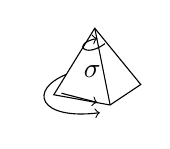
\begin{tikzpicture}[scale=.65]
\draw(0,1.3)--(-.8,0)--(.3,-.2)--(.9,.2)--cycle;
\draw(0,1.3)--(.3,-.2);
\draw[->](-.65,.03)--(.05,-.15);
\draw[->](-.55,.4)..controls(-1.3,.1)and(-1.1,-.5)..(.1,-.35);
\draw[->](.2,1)..controls(-.2,.7)and(-.45,1)..(.05,1.1);
\node at(-.05,.45){$\unsure{\sigma}$};
\end{tikzpicture}}
\mspage{35}
